\section{Results}
\label{sec:result}
In this section, we present the results from our study, beginning with a description of the participants' demographics. This is followed by quantitative and qualitative results regarding cognitive load, and concluded with observations of participants' behaviors. The quantitative measures are directly copied from pen-and-paper surveys and captured through system logs during participant interactions. The interview results are transcribed and coded by the first author, with the codes then grouped into themes. The behavioral data is cleaned and processed, available as open data~\footnote{link-to-github}.

\begin{figure}[h]
    \centering
    \begin{subfigure}[b]{0.65\textwidth}
        \centering
        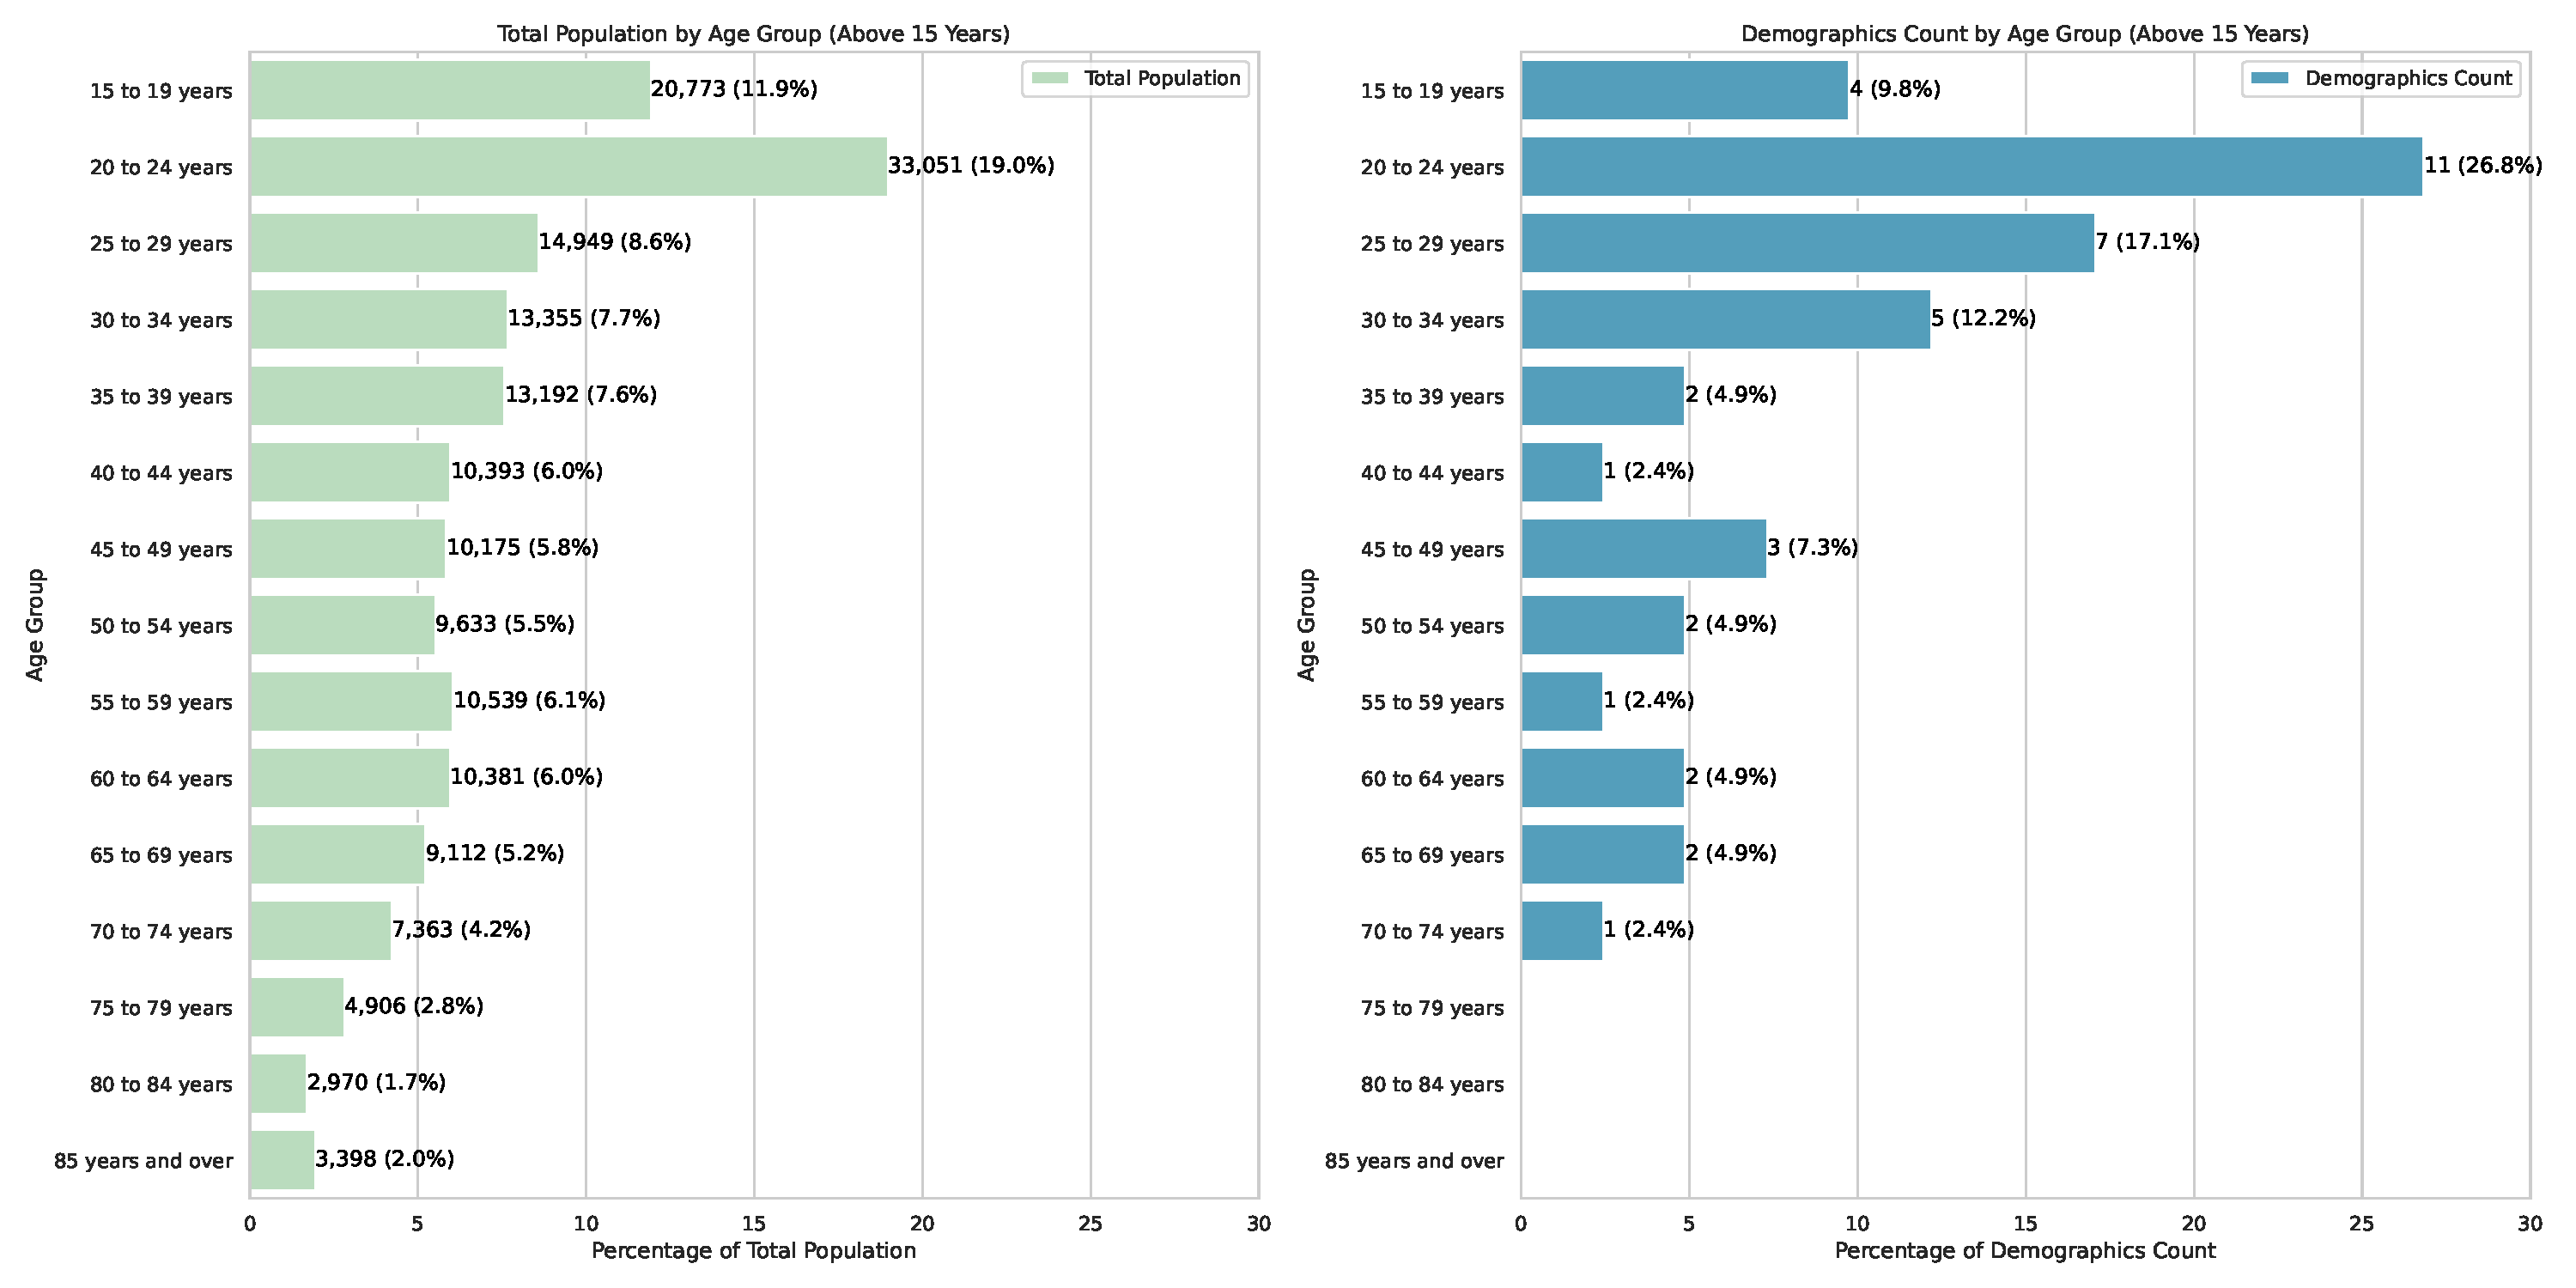
\includegraphics[width=\textwidth]{content/image/demo/demo_age_group.pdf}
        \caption{Age distribution}
        \label{fig:demoAge}
    \end{subfigure}
    \hfill
    \begin{subfigure}[b]{0.3\textwidth}
        \centering
        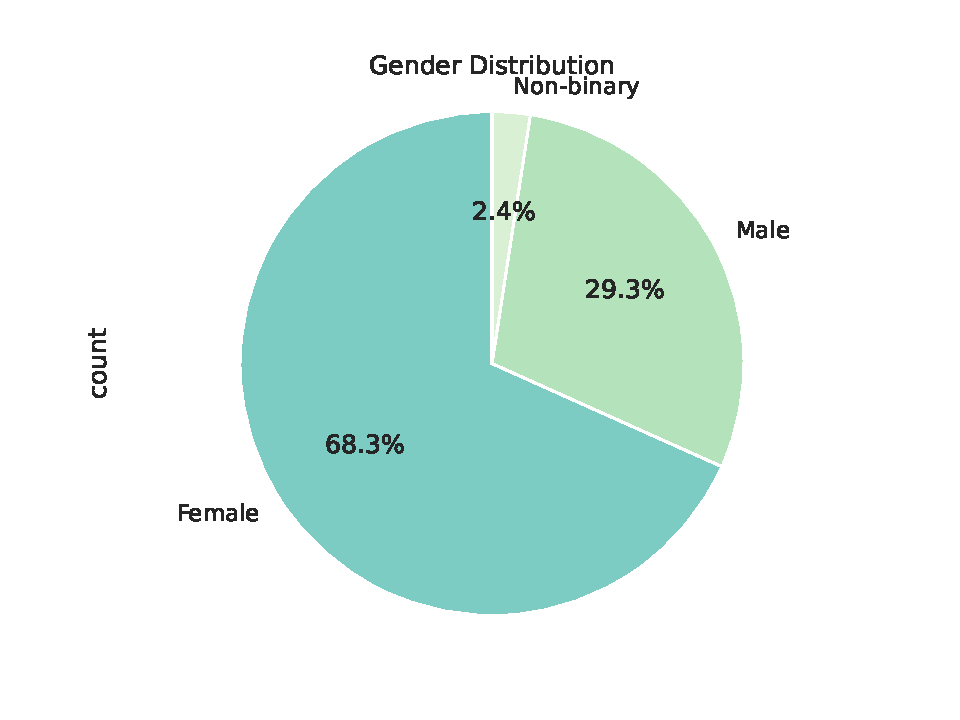
\includegraphics[width=\textwidth]{content/image/demo/demo_gender.pdf}
        \caption{Gender distribution}
        \label{fig:demoGender}
    \end{subfigure}
    \caption{Two figures side by side}
    \label{fig:Demographics}
\end{figure}

% maybe more the figure to the appendix?

\subsection{Demographics}
We recruited a total of $41$ participants, $10$ for each experiment condition. One participant was removed due to data quality concerns. The age of the participants has a mean centered at $34.63$ years old with the full distribution of the participant age distribution to the right of Figure~\ref{fig:demoAge}. The population of the county is presented to the left in the figure. We see that the recruited participants follow closely with the population only missing a few percentages in the $35$-$45$ range making the recruited sample size slightly younger. Recruited participants were more female than male as shown in Figure~\ref{fig:demoGender}.

In terms of ethnicity, $51.2\%$ of the respondents self-identify as White, followed by $26.8\%$ as Asian, $4.9\%$ as Hispanic, and $7.3\%$ as African American. Additionally, $9.8\%$ of participants identify as having mixed ethnicity.

\subsection{Cognitive Load Results}

\begin{figure}[h]
    \centering
    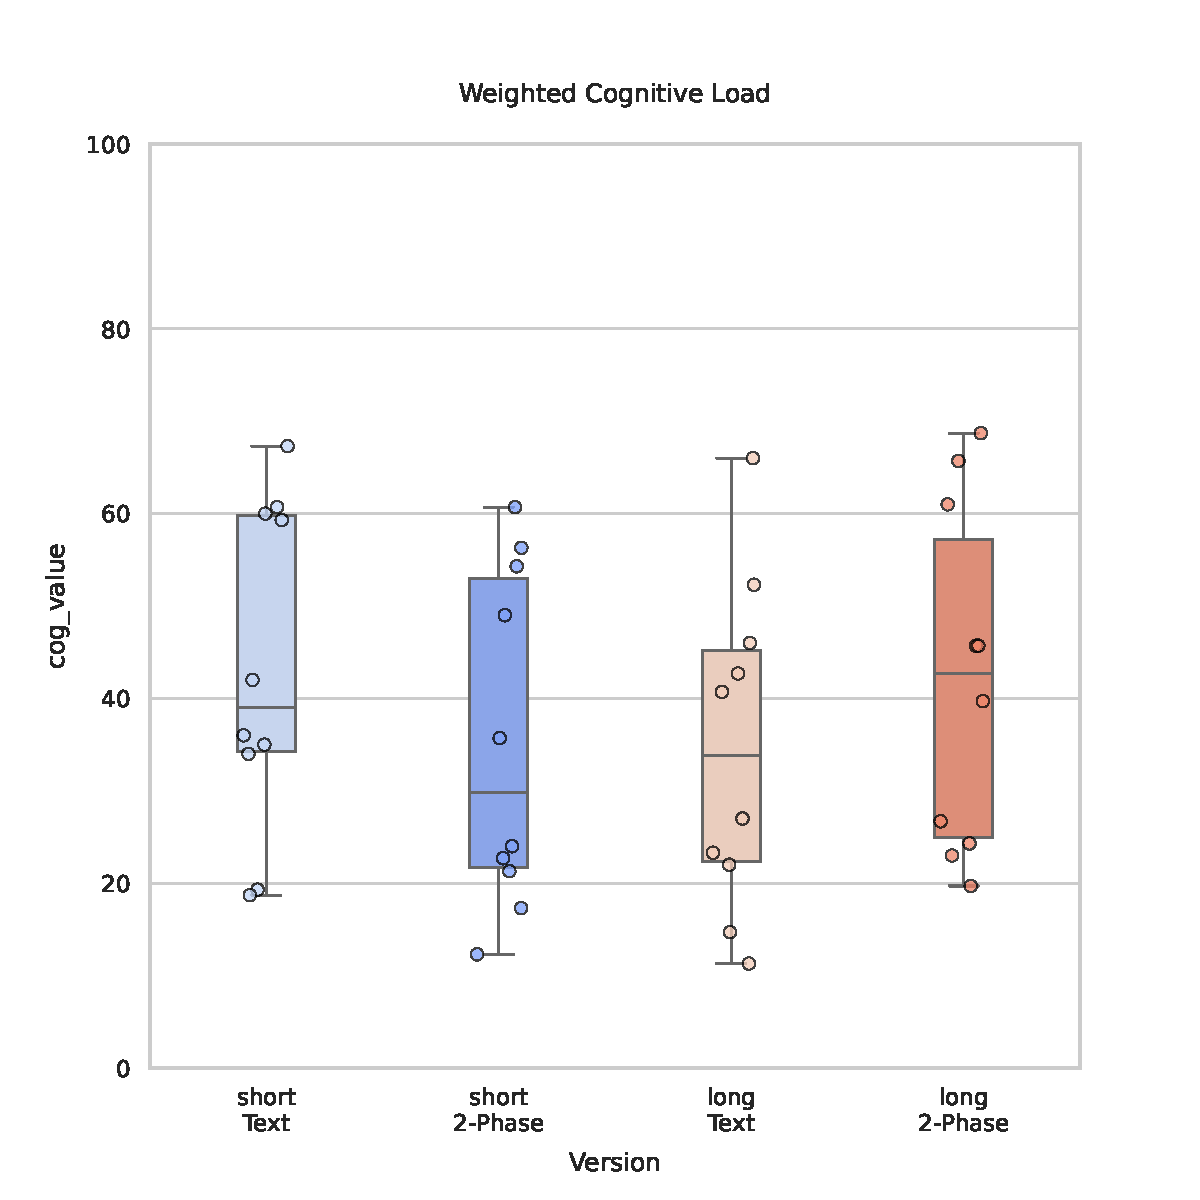
\includegraphics[width=0.5\textwidth]{content/image/results/nasatlx_final_value.pdf}
    \caption{NASA-TLX Results}
    \label{fig:nasatlx-final}
\end{figure}

We show the NASA-TLX weighted results in Figure~\ref{fig:nasatlx-final}. Qualitatively, there is a decrease in cognitive load when comparing short surveys between the text-based interface and interactive interfaces. Conversely, there is an increase in cognitive load when comparing the long survey between the text-based interface and interactive interfaces. However, we are not able to demonstrate statistical significance between the four groups using the Mann-Whitney U test. Reviewing the overall cognitive load, QS participants experienced a `Somewhat High' and `High' cognitive load regardless of length and interface~\cite{hart1988development}. (Need to get the exact percentage).

\begin{figure}[h]
    \centering
    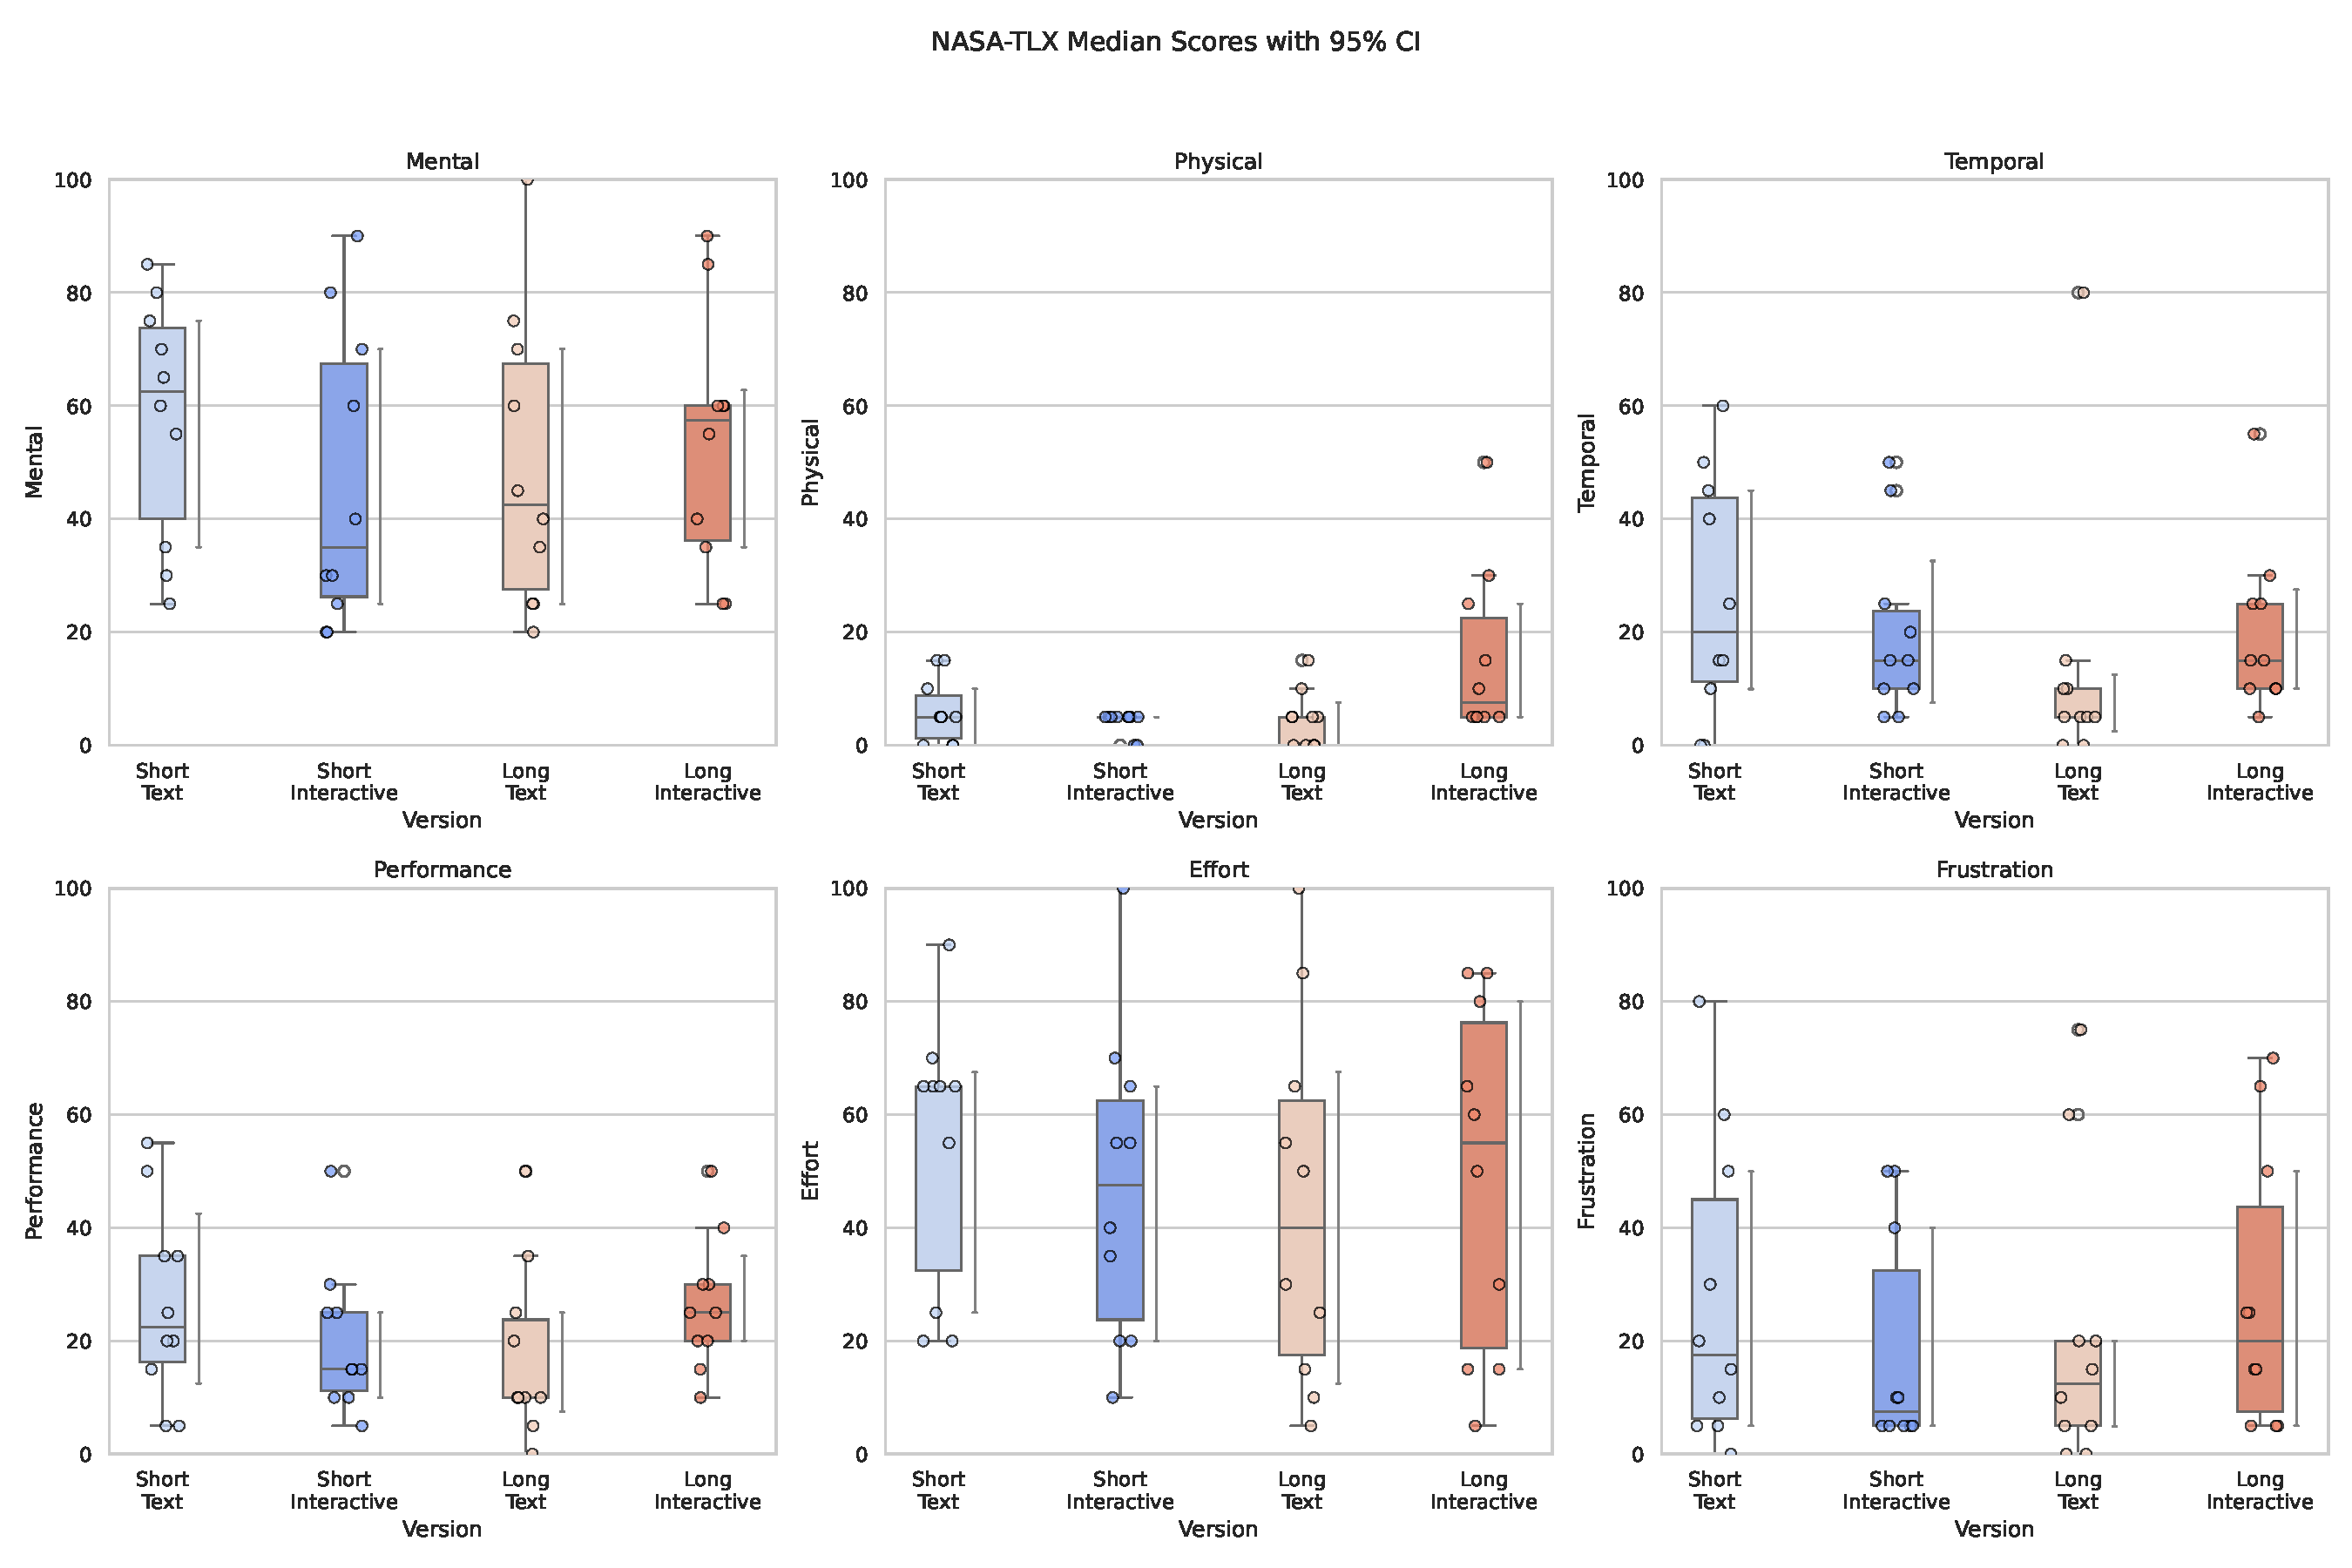
\includegraphics[width=\textwidth]{content/image/results/nasatlx_final_value_with_CI.pdf}
    \caption{NASA-TLX Results}
    \label{fig:nasatlx-with-ci}
\end{figure}

Next, we present the raw scores from the six measurements of NASA-TLX: Mental Demand, Physical Demand, Temporal Demand, Performance, Effort, and Frustration in Figure~\ref{fig:nasatlx-with-ci}. We also show the 95\% confidence interval around the mean for each boxplot.

Mental Demand remains high across all four conditions with a wide variance of responses. The short interactive interface has the lowest median score across all conditions. We see no statistical significance between conditions. For Physical Demand, all conditions except Long Interactive showed minimal scores, with the Long Interactive condition having a noticeably higher median score. There is statistical significance between short and long interactive interfaces ($p<0.01$) as well as text and interactive interfaces in long surveys ($p<0.05$).

Temporal Demand showed more variation across groups. It is interesting to see that the median across the short text interface is among the highest compared to the rest of the groups, while the long-text interface showed the least Temporal Demand. Our statistical tests showed a significant difference between the long text interface and the long interactive interface ($p<0.05$). Performance scores are relatively low across all conditions, indicating that participants experienced less cognitive load from performance. Effort scores echo the mental demand, showing a wide distribution with a high median across the four groups. Lastly, regarding Frustration, we observe qualitatively that the short text interface has a higher median value than the short interactive interface. The opposite is observed in longer surveys, where respondents in the long survey with a text interface experienced less frustration than the interactive version based on median values. We cannot establish statistical significance in the latter three aspects of NASA-TLX.

Based on these results, given the small sample size for each group of participants, we were not surprised that most results do not provide statistical significance in changes in cognitive load values. However, there are some trends that we capture via descriptive statistics. First, comparing the overall cognitive load and the breakdown of the sub-components between text interface and interactive interface across the short survey, we see a general trend in a reduction of cognitive load. Next, we are surprised by the upward trend between the text and interactive interface for the longer list. This is against our original hypothesis that under even complex situations, we should see a clearer portrait of how interactive interactions can reduce cognitive load. While it is possible that interactive interfaces can increase study participants' cognitive load, our qualitative results do not hint at this possibility. In addition, comparing the long and short survey in the text-based interface, it is counter intuitive to see a downward trend across cognitive load. Logically, choosing among more options would demonstrate a higher cognitive load.

These results lead us to further investigate the source of cognitive demands and participants' behaviors.

\paragraph{Mental Demand} This section dissects the sources where participants experienced mental demand.
\paragraph{Physical Demand} This section dissects the sources where participants experienced physical demand.
\paragraph{Temporal Demand} This section dissects the sources where participants experienced temporal demand.
\paragraph{Performance} This section dissects the sources where participants experienced performance.
\paragraph{Effort} This section dissects the sources where participants experienced effort.
\paragraph{Frustration} This section dissects the sources where participants experienced frustration.

\subsection{Interaction Behavior Analysis}
To further investigate the cognitive load results, we focused on participants' behaviors during the survey. Specifically, we aim to understand the time participants spent on the options as well as when a participant makes changes to the survey. When a study participant clicks their mouse on the interface to complete some action, whether it is a drag-and-drop, updating votes, or placing options into a specific group, a timestamp and the payload of the update are stored in the log. The time difference between two actions is attributed to the time the participant took to decide and enact upon a behavior. While participants can be thinking about other things, this is the best proxy we have to study participant behaviors.

\begin{figure}[h]
    \centering
    \begin{subfigure}[b]{0.32\textwidth}
        \centering
        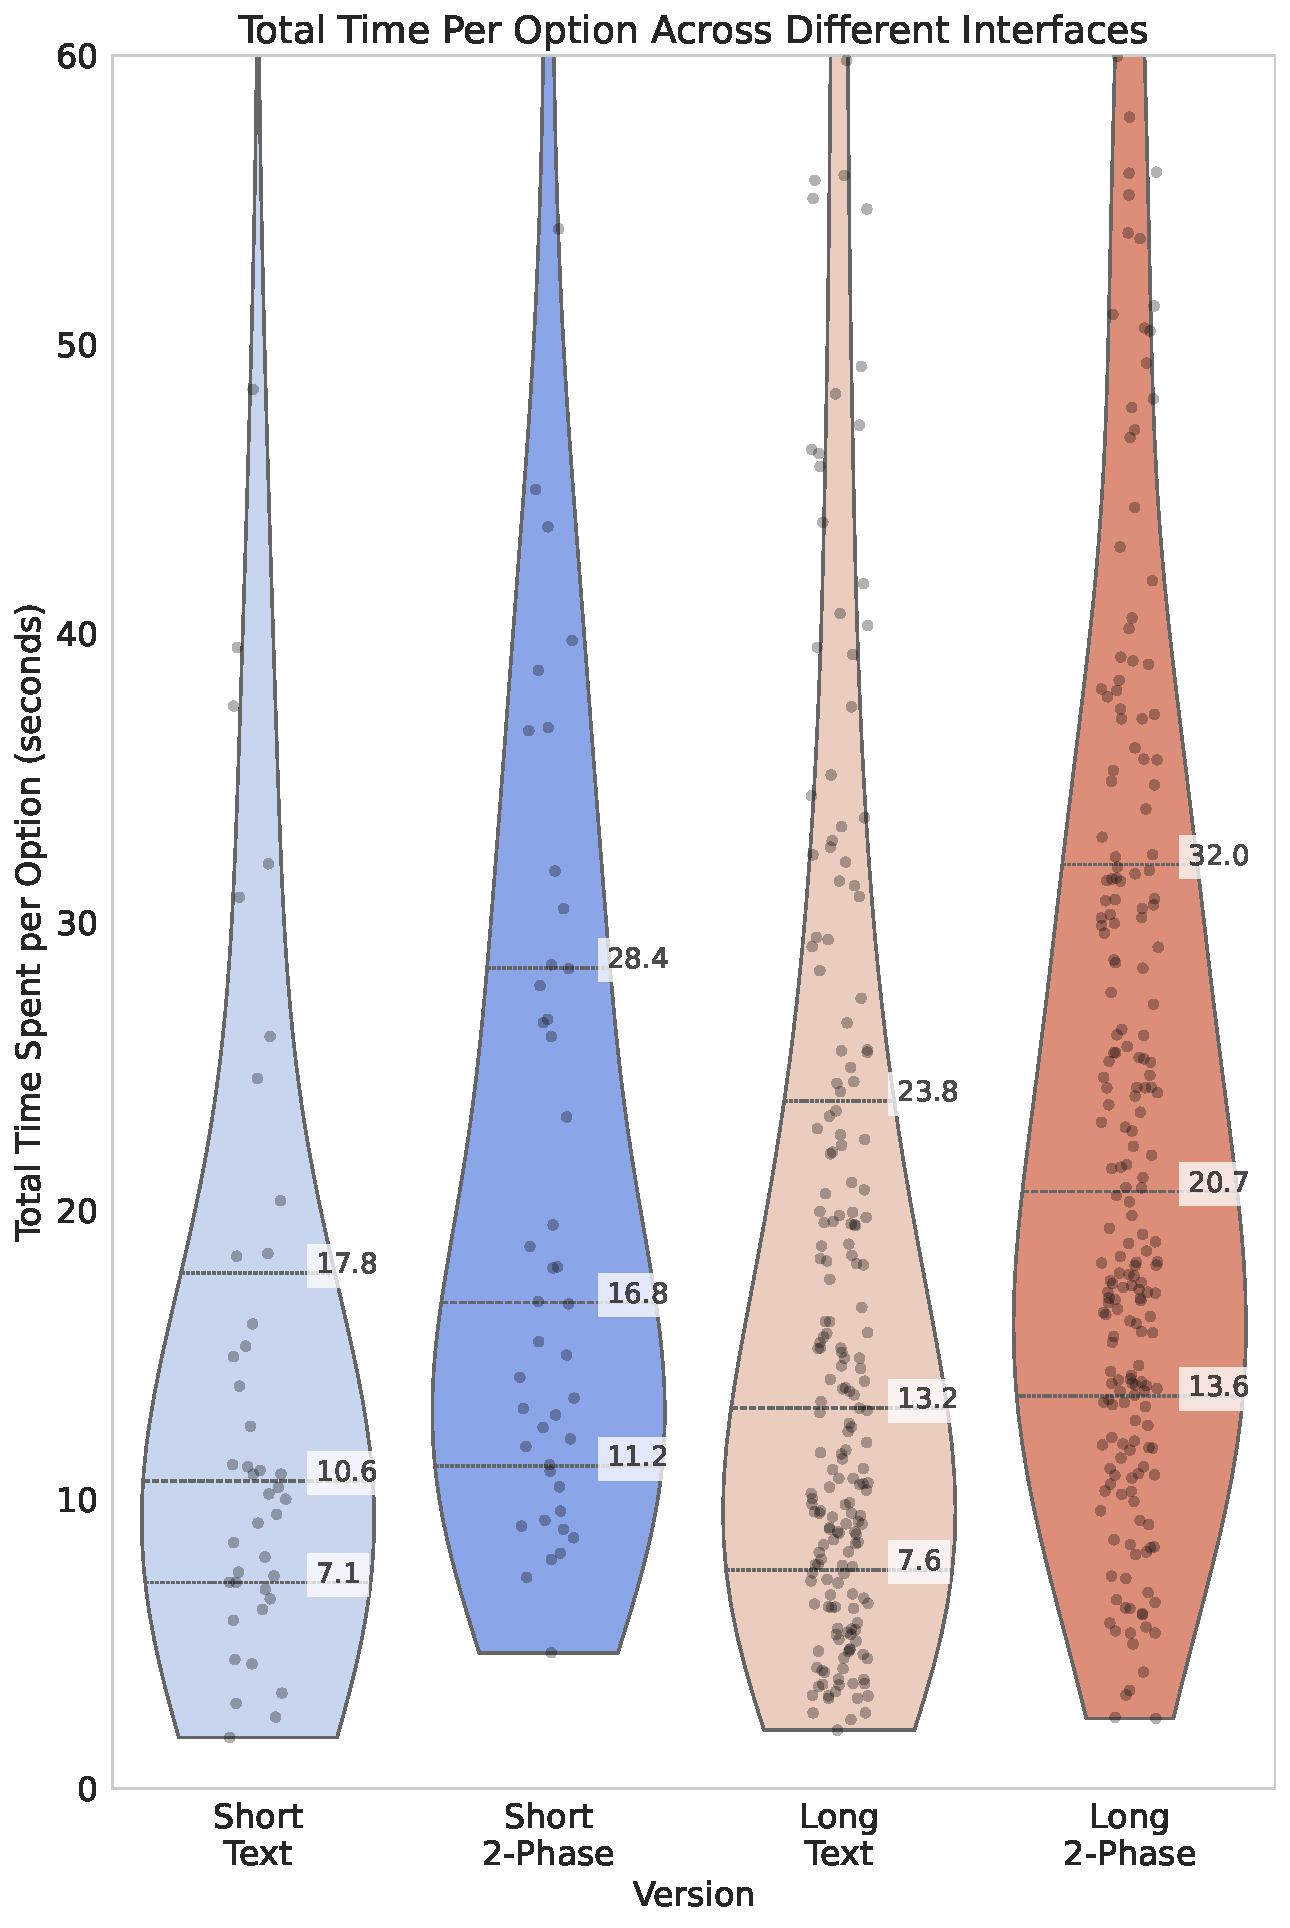
\includegraphics[width=\textwidth]{content/image/results/total_time_per_option.pdf}
        \caption{Total Time per option}
        \label{fig:total_time}
    \end{subfigure}
    \hfill
    \begin{subfigure}[b]{0.32\textwidth}
        \centering
        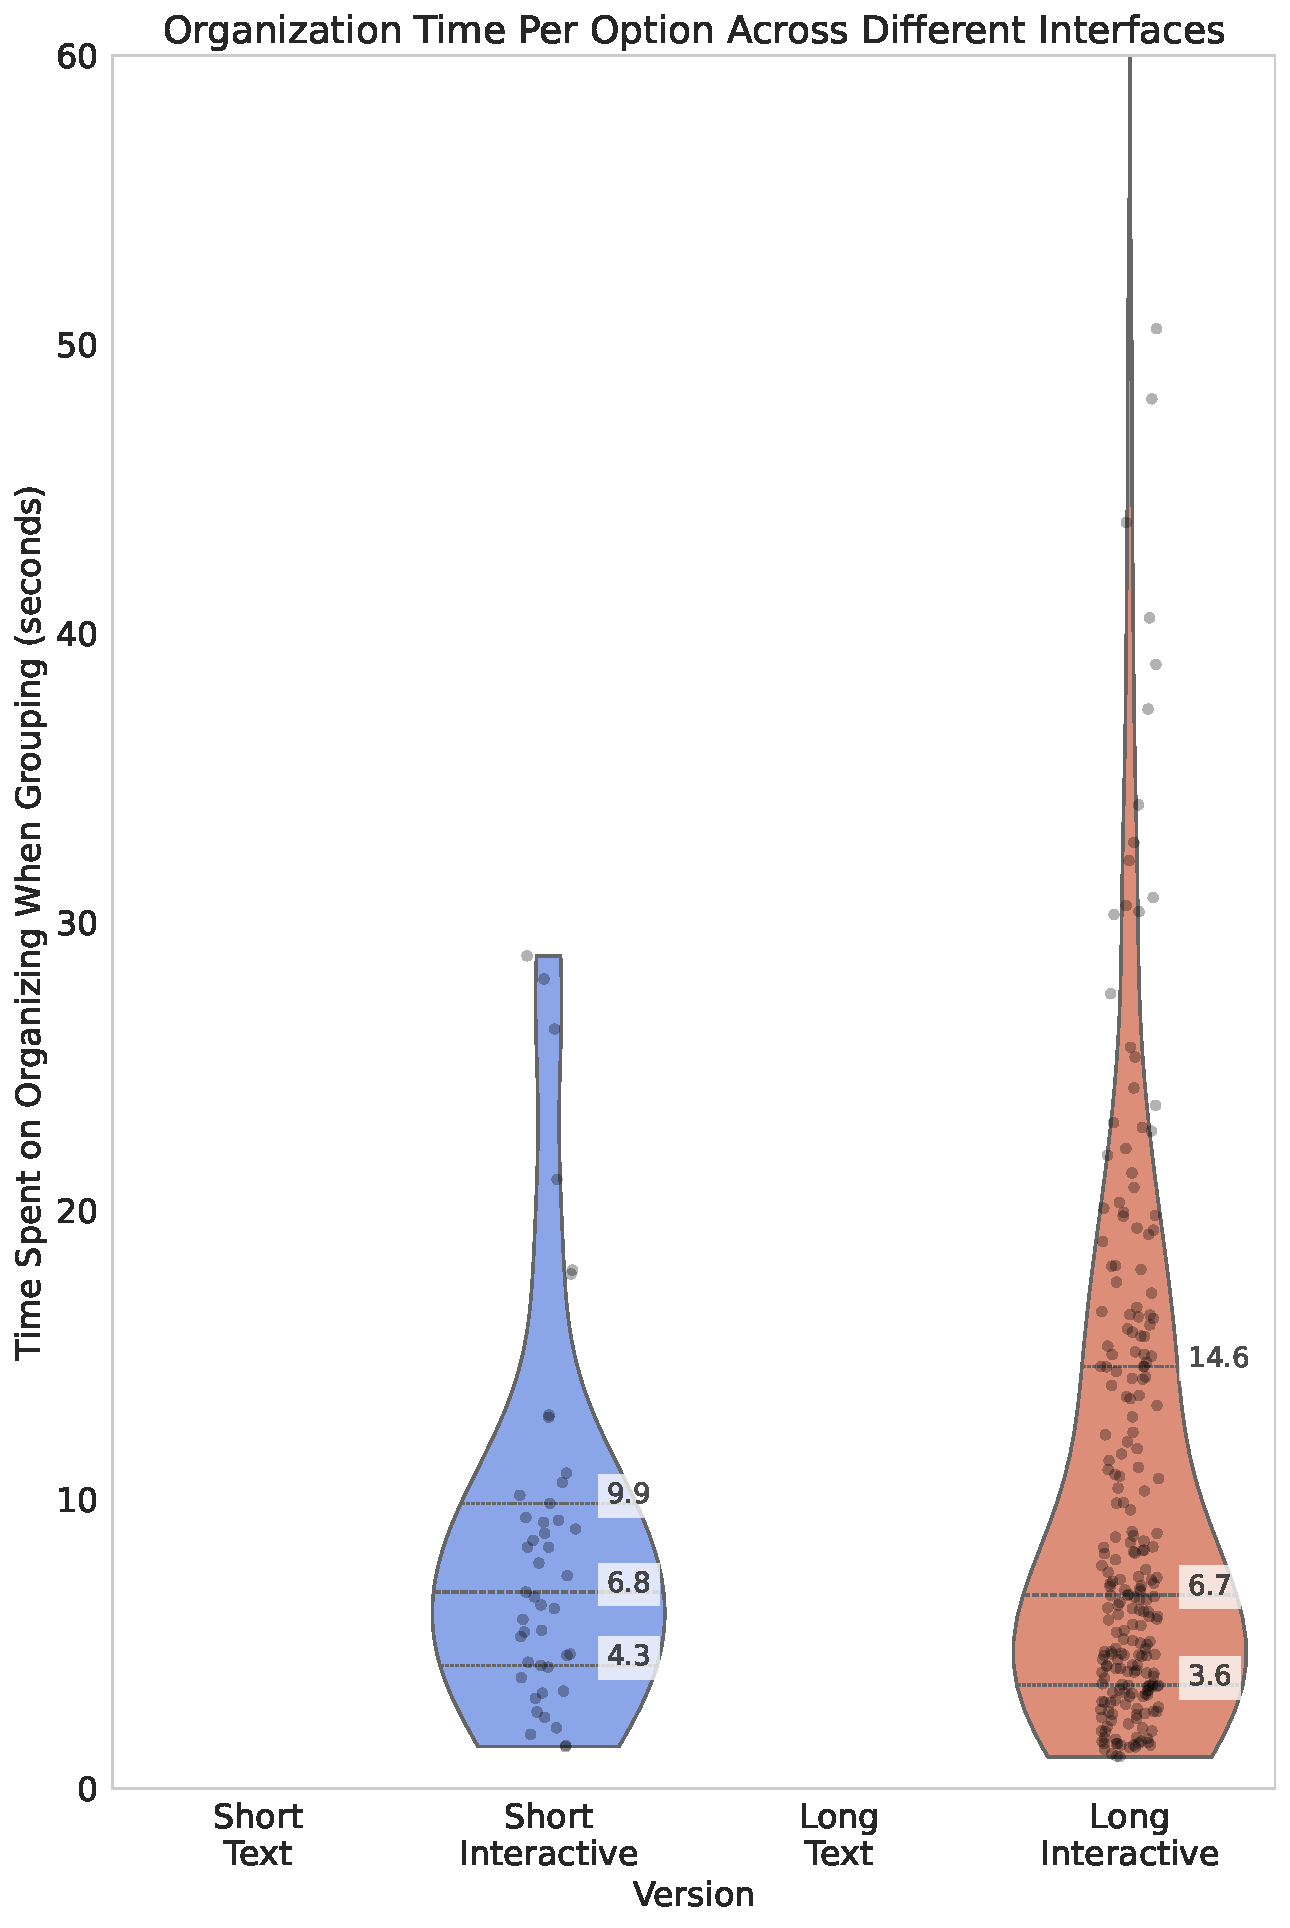
\includegraphics[width=\textwidth]{content/image/results/org_time_per_option.pdf}
        \caption{Organization Time per option}
        \label{fig:org_time}
    \end{subfigure}
    \hfill
    \begin{subfigure}[b]{0.32\textwidth}
        \centering
        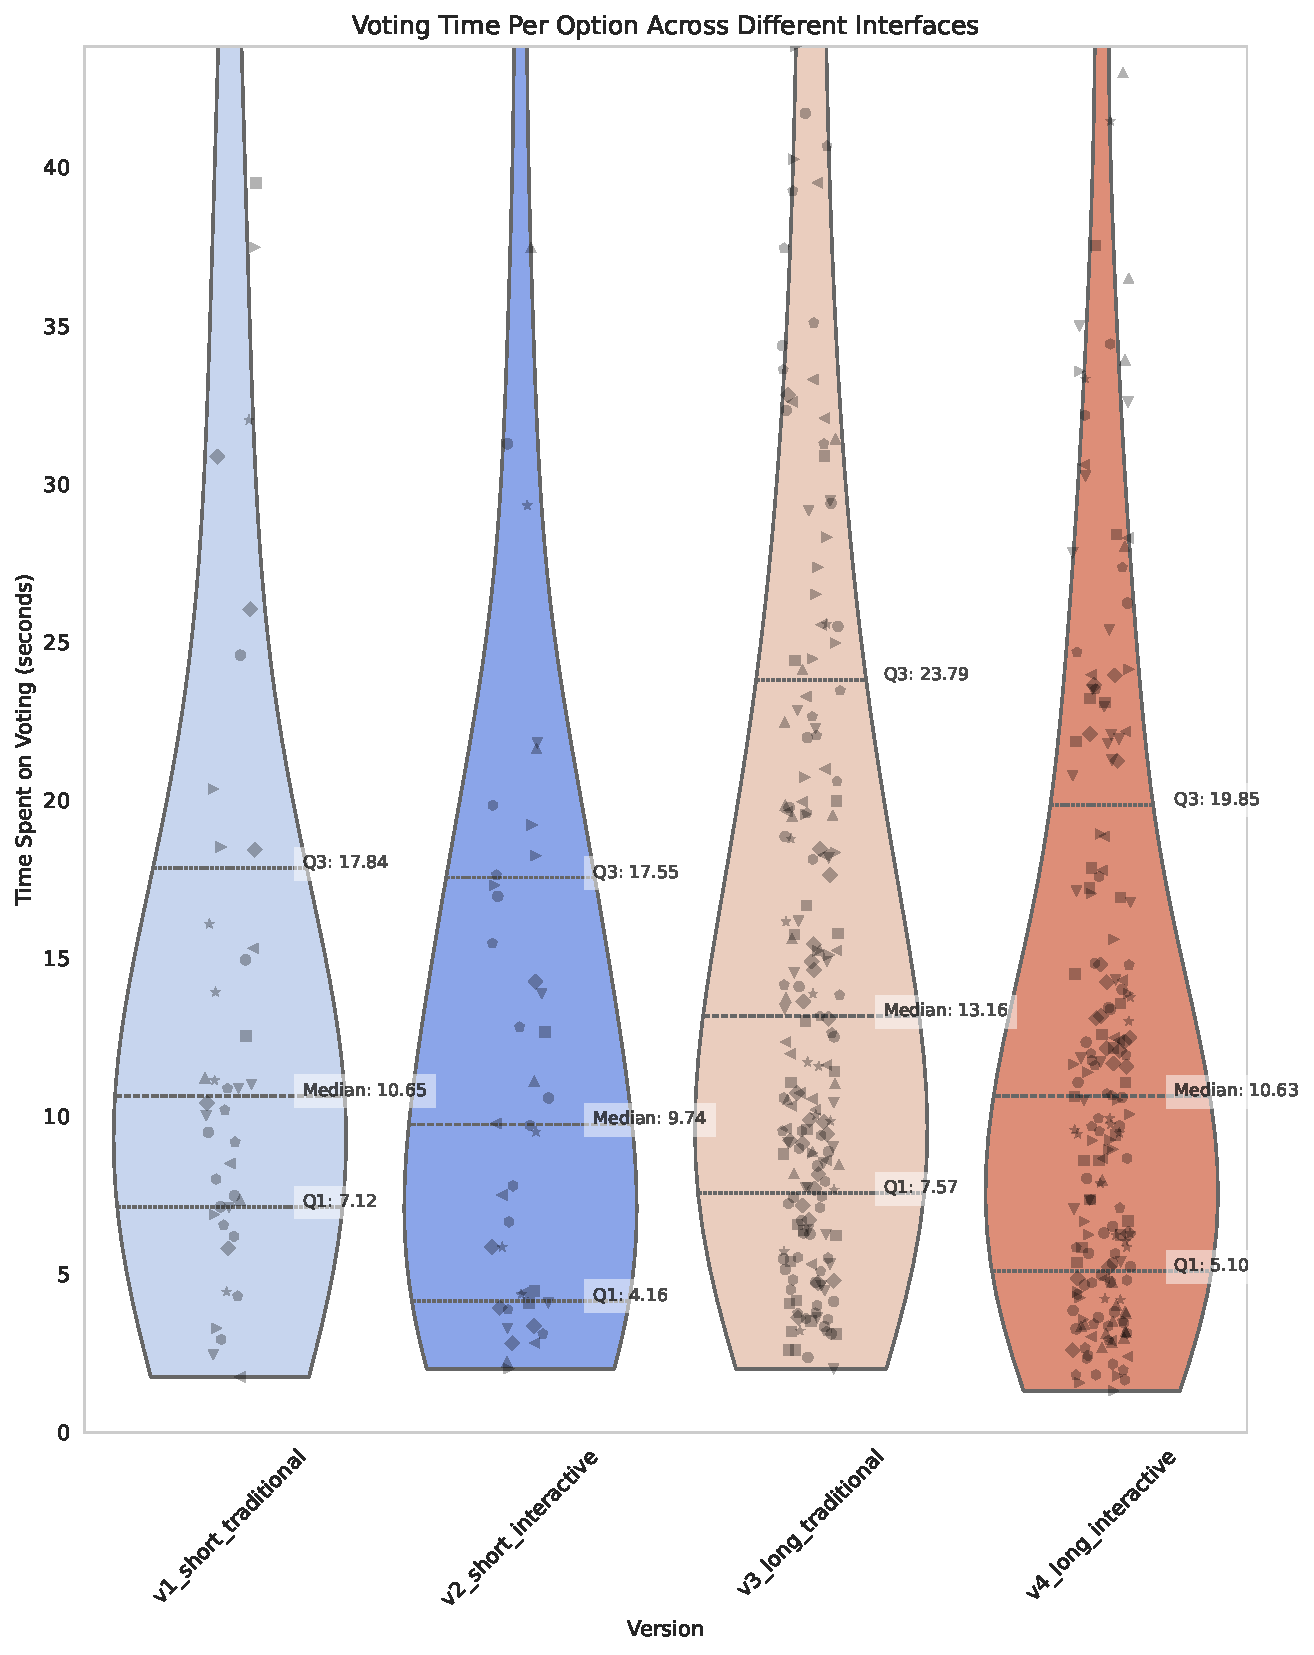
\includegraphics[width=\textwidth]{content/image/results/voting_time_per_option.pdf}
        \caption{Voting Time per option}
        \label{fig:vote_time}
    \end{subfigure}
    \caption{Breakdown of time per option}
    \label{fig:Time Spent Per Option Per Person}
\end{figure}

\subsection{Time Spent per Options}
First, we define time spent per option. A participant can enact several actions related to the same option, for example, a participant might spend $t_1$ time to place the option into a `lean positive' category; spend $t_2$ and $t_3$ time to drag and drop the options to reposition it on the interactive interface; spend $t_4$ and $t_5$ time to update the upvotes on that option. In this case, we would define voting time as $t_4 + t_5$ for that option, and organization time as $t_1 + t_2 + t_3$.

To reduce noise, we intentionally drop all the time participants spent on the first option in the organization phase or voting phase. The goal is to reduce the inclusion of time they spent on reading the prompt, forming their preference, or understanding the interface. We present the results in Figure~\ref{fig:Time Spent Per Option Per Person} where each of the dots represents the time accumulated for an option that a participant interacted with. The violin plot shows the distribution of the dots and the three horizontal lines represent the median, 25th percentile, and 75th percentile of the time spent for that interface.

In Figure~\ref{fig:total_time}, we observe that participants spent more time on the interactive interface than the text interface in both short and long surveys. A non-parametric statistical test supports such observation with $p<0.01$ for short and $p<0.0001$ for long surveys. This is not surprising because participants need to review the options and organize them in the interactive interface which takes more time. We break down the total time spent into organization time and voting time in Figure~\ref{fig:org_time} and Figure~\ref{fig:vote_time}.

Once we separate the organization time (Figure~\ref{fig:org_time}) and identify the voting time (Figure~\ref{fig:vote_time}), while there are no statistically significant differences between the text interface and the interactive interface in the short survey, we see a statistically significant reduction ($p<0.01$) in voting time between the text interface and the interactive interface. In other words, our original hypothesis holds in which the two-step design process did facilitate participants in making their decisions.

\begin{figure}[h]
    \centering
    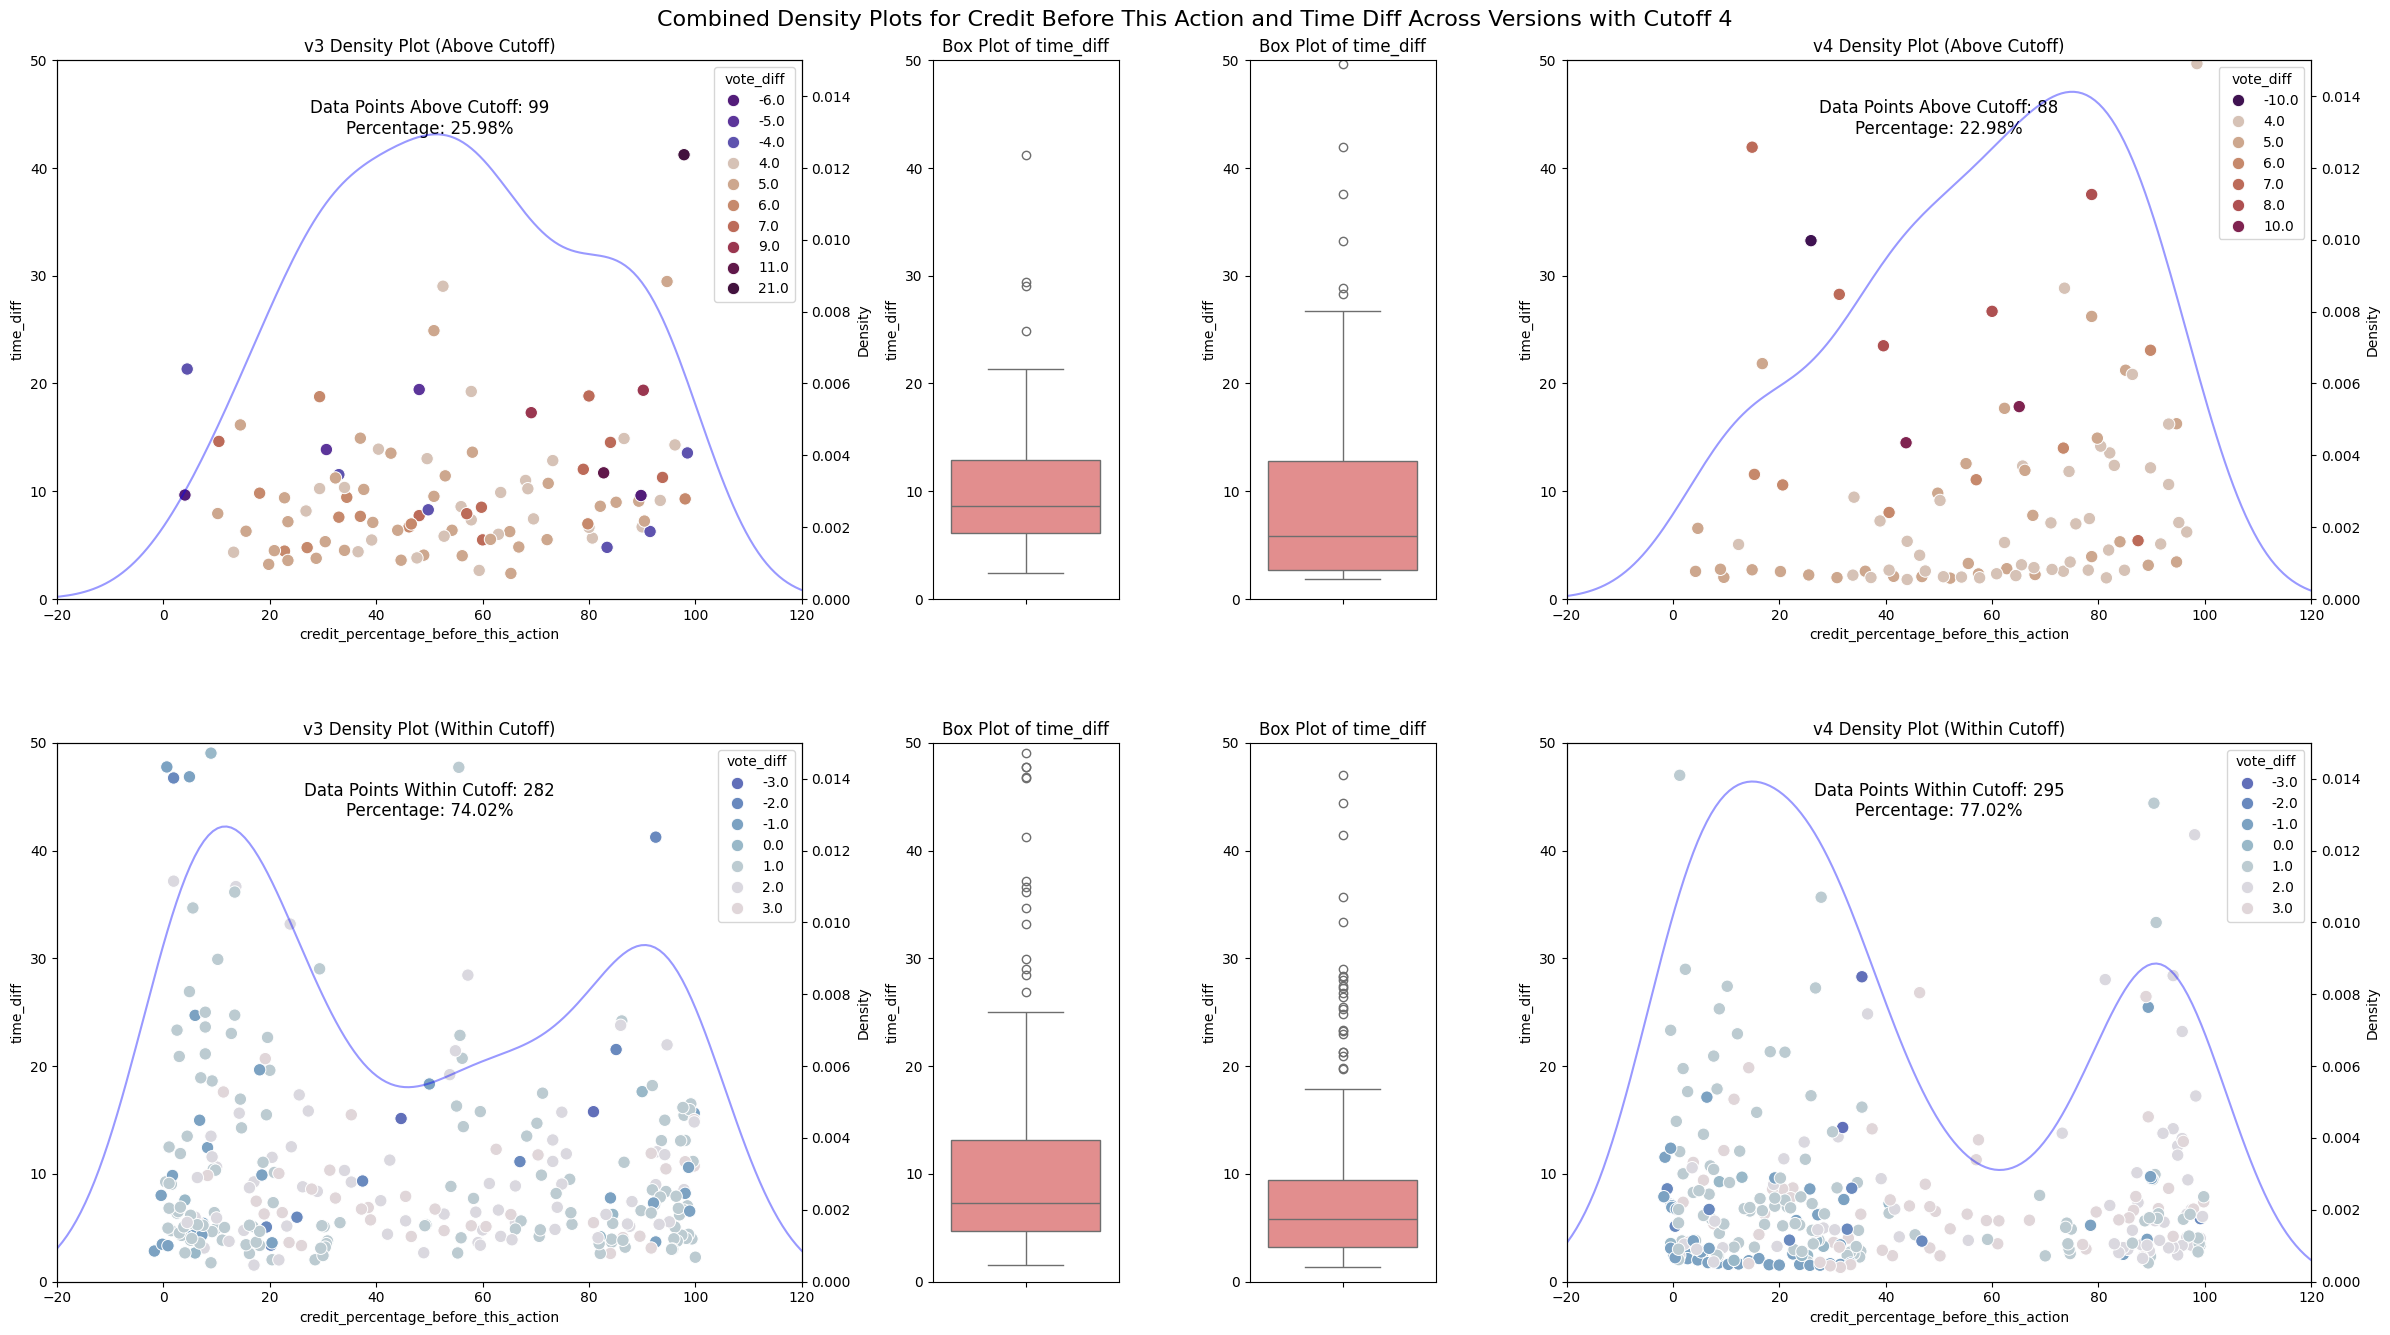
\includegraphics[width=\textwidth]{content/image/results/temp_cut4.png}
    \caption{Breakdown of voting actions (needs to update chart text)}
    \label{fig:voting_v3_v4}
\end{figure}

\subsection{Budget and Voting Behaviors}
Next, we examine participants' voting behavior and how it changed throughout the progress. Given that we observe significant differences in voting time changes comparing text interface and interactive interface for the long option survey, we focus on deciphering the voting action changes between these two experiment conditions in this subsection.

Figure~\ref{fig:voting_v3_v4} plots the time of voting actions over the remainder of the participant's budget across the text and interactive interface. In other words, different from~\textcite{quarfoot2017quadratic} focusing on the number of accumulated votes over an individual's time, where they showed QV voters make more revisions than Likert Surveys, we focused on the budget scarcity which can influence QS respondents' behaviors.

We further separated the behaviors where participants made bigger changes or smaller changes to the option. In this figure, we define an adjustment of four or more votes as a large adjustment which we plotted in the first row of the Figure. Adjustments of three or fewer votes are considered small adjustments.

First, the plot demonstrated a clear cluster of voting actions in the bottom left corner of the interactive interface for small vote adjustments. In other words, participants made much smaller but more rapid adjustments when their budgets were running low. Second, larger adjustments are made when the participants have more options comparing the two plots on the first row. We interpret this behavior as participants in the interactive interface have constructed a clearer image of option preferences and, hence, have the ability to take larger strides in allotting their budget and deciding the number of votes at the beginning of the survey. Toward the end, participants using the interactive interface are then making fine-tuned adjustments to ensure that their preferences are reflected in their submissions.

% add qualitative support

\subsection{Interface Comments}
Finally, we present the qualitative responses related to the interface design and their experience working with QS across all experiment groups.

\paragraph{Organization is required and beneficial}
Many participants (N=7) who responded to QS using the interactive interface expressed the helpfulness of the organization phase proactively when asked what they liked about the interface in general. In fact, half of the participants (N=5) in the long interactive interface group expressed such an opinion. Multiple participants (N=4, 3 from long interactive interface group) felt that the upfront introduction of all the topics allowed them to process and think about the full picture, thereby digesting all the information more comprehensively. 

\begin{displayquote}
I would say that (the interface) definitely (supported me), by being able to have a preliminary categorization of all the topics. First, it introduced me to all the topics, so that I can think about them like I can just kind of leave it there in my head space to think about and process \bracketellipsis So being able to digest all the information prior to actually allocating the budget or completing the quadratic survey.

\noindent \hfill -- S009, long interactive interface.
\end{displayquote}

% \begin{displayquote}
% \bracketellipsis having some sort of categories helped in establishing these 3 categories is like the first tip, and then, like I said, I have other categories myself~\bracketellipsis classifying things into categories~\ldots\ make me~\ldots\ I don't know \ldots\ It was just easier for me. 

% \noindent \hfill -- S021, long interactive interface.
% \end{displayquote}

Participants (N=4, 2 from long interactive interface group) mentioned that organization support them to allot the intensity of votes by helping them focus and prioritize options through ranking options. This excercise allows them to follow a clear decision making process that avoids confusion.

\begin{displayquote}
If I had to choose a number like that in the beginning. That would have been really bad, but positive, neutral, negative. That was good enough.

\noindent \hfill -- S016, long interactive interface.
\end{displayquote}

\begin{displayquote}
I think \ldots\ ranking at the beginning one's impression towards these issues helps to like determine how many votes should be put towards them. 

\noindent \hfill -- S002, short interactive interface.
\end{displayquote}

Last, one participants highlighted the one-at-a-time approach during the organization phase allowed thoughtful reflection to think about their attitude toward that option.

\begin{displayquote}
Like, at the moment (during organization), when it gives you, like, rank it if it's positive or neutral or negative~\bracketellipsis it gives you time to just focus on that single thing and rank it based on how you feel at that moment.
    
    \noindent \hfill -- S013, short interactive interface.
\end{displayquote}

We see a call for organizational features proactively when asking participants using the text-based interface what features they wanted from the interface. Almost half of the participants (N=4) using the long text interface expressed some form or another that can help reduce the decision space when responding to the QS.

\begin{displayquote}
    If anything, I think I would like to be able to like, click and drag the categories themselves so I could maybe reorder them to like my priorities.
        
        \noindent \hfill -- S025, long interactive interface.
\end{displayquote}

\begin{displayquote}
    Because with this many (options), especially when I'm thinking \ldots\ Ok, where was (the option) \ldots\ Where was (the option) you know? Oh, that's right. Maybe I could give another up another upvote to the, you know whatever~\bracketellipsis
        
        \noindent \hfill -- S028, long interactive interface.
\end{displayquote}

\paragraph{Direct Manipulation Enhances Reflective Decision-Making}
As the proximity of position are mostly determined by the categorization in the first phase of the interactive interface. Several participants mentioned how they used direct Manipulation in the software as a process for reflective thinking upon their decision making process. One participant mentioned:

\begin{displayquote}
So I tried to make a ranking~\bracketellipsis and by creating this ranking, by dragging the related issues~\ldots\~i don’t know~\ldots\~that helped me organize my ideas.
    
\noindent \hfill -- S021, long interactive interface.
\end{displayquote}

\begin{displayquote}
I think the system was actually really helpful because I could just drag them.~\bracketellipsis Because when I was unsure, because if I couldn't drag them then I couldn't compare 2 options very well like side to side, because because this is pretty long list~\ldots\ so if I couldn't drag it, then I would have a harder time organizing my thoughts, whereas  with the dragging feature I can really compare them, I can drag this one up here, and then compare it to the top one versus like not being able to track it at all
    
\noindent \hfill -- S039, long interactive interface.
\end{displayquote}


But more importantly, it acts as a process for reflective verification and iterative decision making. These can include post reflection after expressing the intesnsitve of preferences, or a preperation to decide on number of votes for the next option.


\begin{displayquote}
So I would give the votes, and then I would drag and drop.~\bracketellipsis So I guess to see what my ranking look like. And see if I could give more money or not.
    
\noindent \hfill -- S021, long interactive interface.
\end{displayquote}

\begin{displayquote}
\bracketellipsis this is something that's really important to me \ldots\ So I had the flexibility to move it to positive. So just having the kind of like shift in perception. ~\bracketellipsis especially because when I was doing categorize categorization in the first step, ~\bracketellipsis what I thought about it in the moment. ~\bracketellipsis In the second step there was a shift in my perception of the issue just reflecting. So being able to change. That was really nice as well. 

\noindent \hfill -- S009, long interactive interface.
\end{displayquote}

Conversely, in the text interface, one participant proactively mentioned a request to add click and drag functionalities to the interface. The participants described such function to group by topic categorization and also priority placement through direct manipulation. 

\begin{displayquote}
If anything, I think I would like to be able to like, click and drag the categories themselves so I could maybe reorder them to like my priorities. And so I could maybe make that like a descending or ascending like list of like importance.~\bracketellipsis if I could pull that up to the top, say myself like click and drag it up there, I think then I would stack the things I think it would affect under it. So like, I would put then, like youth, pro-education programs and adult education and early childhood programs and kinda stack those altogether.~\bracketellipsis I would hope that money would trickle down and also increase all the rest of those things. So I would put less upvotes in there because I would hope to dribble out effect would kick in.~\bracketellipsis I would kind of make myself categories and subcategories out of this list. If I could organize it.

\noindent \hfill -- S025, long text interface.
\end{displayquote}

% Ti-Chung Cheng: So what elements of the software interface do you dislike, or like the most, if any, when expressing your preferences on responding to societal issues?
% S009: Hmm! What I like the most actually, probably the sorting function. I think that it really helped me organize my thoughts really, clearly, in terms of what I would dislike the most. really, not that much. I would say. yeah, also, like how we could categorize it, like even within the voting stage rather than just at the categorization stage. 

% Ti-Chung Cheng: Can you tell me a little bit more about the screen? How did the vertical screen help you?
% S037: I think because it helps the layout of, because it's like a long 3 bar. So it's easier for you to to drag and drop, and you can actually sort it, judging by the votes. But I do not do that. But I think this layout is could be helpful in that aspect.
**



